\documentclass[10pt,a4paper]{article}
\usepackage[utf8]{inputenc}
\usepackage[english]{babel}
\usepackage[T1]{fontenc}
\usepackage{amsmath}
\usepackage{amsfonts}
\usepackage{amssymb}
\usepackage{subcaption}
\usepackage{makeidx}
\usepackage{graphicx}
\usepackage{fourier}
\usepackage{listings}
\usepackage{color}
\usepackage{hyperref}
\usepackage[left=2cm,right=2cm,top=2cm,bottom=2cm]{geometry}
\author{Tommy Müller, Marcus Dittrich, Vincent Noculak}
\title{Zeeman-Effekt}

\lstset{language=C++,
	keywordstyle=\bfseries\color{blue},
	commentstyle=\itshape\color{red},
	stringstyle=\color{green},
	identifierstyle=\bfseries,
	frame=single}
\begin{document}

\maketitle
\newpage
\tableofcontents
\newpage

\section{Theorie}

\section{Durchführung}

In dem Versuch sollte der normale Zeeman-Effekt beobachtet werden. Abbildung \ref{aufbau} zeigt den Aufbau des Versuchs. Mit Hilfe einer Quecksilber-Spektrallampe, die sich für Teile der Messung in einem Magnetfeld befindet, wird Licht erzeugt. Dieses wird durch eine Sammellinse gebündelt und durch einen Monochromator geleitet, mit dessen Hilfe bestimmte Spektrallinien des Lichts gezielt durchgelassen werden können. Das vom Monochromator durchgelassene Licht läuft dann durch eine Linse, gefolgt von einem Fabry-Perot-Interferometer. Durch eine Kamera kann das Licht nach dem Fabry-Perot-Interferometer am Computer untersucht werden. 

Der Versuch begann damit, das Spektrum der Quecksilber-Spektrallampe bei noch ausgeschaltetem Magnetfeld mit Hilfe des Monochromators zu beobachten. Daraufhin wurde unter Beobachtung der grünen Spektrallinie der Strahlengang auf optimale Schärfe justiert. Hierzu wurden die vom Fabry-Perot-Interferometer erzeugten Ringe betrachtet und darauf hin aufgenommen.

Jetzt wurde das Magnetfeld angeschaltet, um den normalen Zeeman-Effekt zu untersuchen. Ausgehend von der grünen Spektrallinie, wurde die Polarisation der Zeeman-Komponenten und die Aufspaltung der Spektrallinie abhängig von der Stärke des Magnetfelds beobachtet.

\begin{figure}[h]
	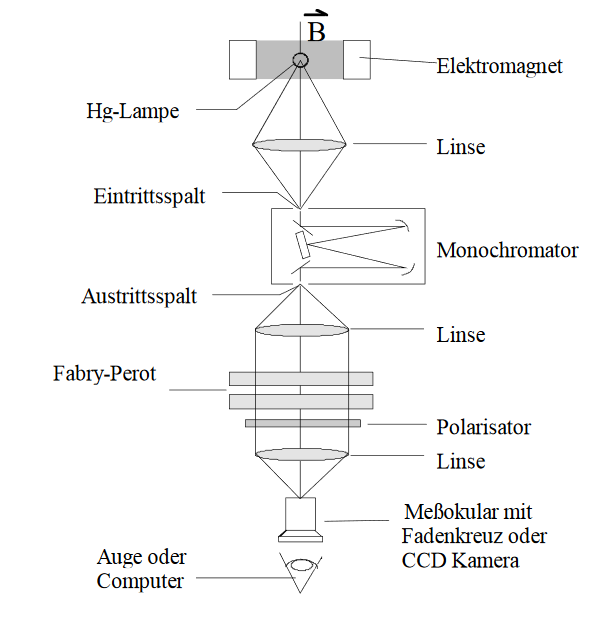
\includegraphics[scale = 1]{Zeeman_aufbau.png}
	\centering
	\caption{Versuchsaufbau, Quelle: Versuchsanleitung vom Zeeman-Effekt-Versuch des Fortgeschrittenenpraktikums}
	\label{aufbau}
\end{figure}

\section{Versuchsergebnis}

Mit dem Monochromator hatten wir zum Beginn des Versuchs das Feinstrukturspektrum der Quecksilber-Spektrallampe von $400nm$
bis $900nm$ beobachtet. An dem Monochromator konnte per Rad die durchgelassene Wellenlänge eingestellt werden. Eine Angabe zu der Durchlassgenauigkeit des Monochromators konnten wir nicht finden. In Tabelle \ref{spektrum} können die von uns beobachteten Spektralfarben gesehen werden. Wir waren in der Lage, die meisten Spektralfarben mit einer Abweichung von höchstens 4 Nanometern wahrzunehmen. Die cyanfarbige und rote Spektrallinie konnten wir nicht beobachten. Es fällt auf, dass die von uns beobachteten Spektrallinien immer ein paar Nanometer über den tatsächlichen Literaturwerten gemessen worden sind. Dies könnten an einem systematischen Fehler am Monochromator liegen.

Die bei $577nm$ und $579nm$ liegenden orangenen Spektrallinien der Spektrallampe konnten wir nur als einzelne Linie bei $580nm$ wahrnehmen.

\begin{table}[h!]
	\centering
\begin{tabular}{|l|r|c|lrp{16cm}}\hline
	Farbe & Literaturwerte in nm & Beobachtete Wellenlängen in nm\\\hline
	Violett & 405 & 409\\
	Blau & 436 & 439\\
	Cyan & 492 & -\\
	Grün & 546 & 548\\
	Orange & 577 & 580\\
	Orange & 579 & 580\\
	Rot & 615 & -\\\hline
\end{tabular}
	\caption{Beobachtete Spektrallinien der Quecksilber-Spektrallampe}
	\label{spektrum}
\end{table}

\section{Auswertung}

\section{Diskussion}


\end{document}